%%%%%%%%%%%%%%%%%%%%%%% file template.tex %%%%%%%%%%%%%%%%%%%%%%%%%
%
% This is a general template file for the LaTeX package SVJour3
% for Springer journals.          Springer Heidelberg 2010/09/16
%
% Copy it to a new file with a new name and use it as the basis
% for your article. Delete % signs as needed.
%
% This template includes a few options for different layouts and
% content for various journals. Please consult a previous issue of
% your journal as needed.
%
%%%%%%%%%%%%%%%%%%%%%%%%%%%%%%%%%%%%%%%%%%%%%%%%%%%%%%%%%%%%%%%%%%%

\documentclass[12pt]{iopart}
% \documentclass[10pt]{iopart}
\usepackage[numbers,sort&compress]{natbib}
\def\newblock{\ }
\usepackage{bm}
\usepackage{graphicx}   % need for figures
    \graphicspath{{10_Figures/}}
\usepackage{verbatim}   % useful for program listings
\usepackage{xcolor}      % use if color is used in text
\usepackage{subfigure}  % use for side-by-side figures
\usepackage{hyperref}   % use for hypertext links, including those to external 
% % documents and URLs

\usepackage{tikz}
    \usetikzlibrary{spy,intersections}
\usepackage{etoolbox}
\usepackage{pgfplots}
\pgfplotsset{compat=newest} 

\makeatletter
%\def\cl@chapter{\cl@chapter \@elt {theorem}}%bug in class
\def\cl@chapter{\@elt {theorem}}
\makeatother

\usepackage[capitalize]{cleveref}

\usepackage{xfrac}

\usepackage{siunitx}
    \DeclareSIUnit\Vrms{\volt_{rms}} % volt RMS
    \DeclareSIUnit\fps{fps} % frames per second
    \DeclareSIUnit\MS{\mega S\per\second} % frames per second


    \input{05_Helpers/10_commands.tex}

%
\begin{document}

\title[Rotation Measurement of Particles with an Optial Tweezer]{Rotational 
Speed Measurements of Small Spherical Particles driven by Acoustic Viscous 
Torques utilizing an Optical Trap}

\author{Andreas Lamprecht$^1$, Christoph Goering$^1$\footnote{A.L and C.G.  
contributed equally to this work}, Iwan A.T. Schaap$^2$, Jurg Dual$^1$}

\address{$^1$ ETH Zurich, Institute for Mechanical Systems, Tannenstr 3, 8092 
Zurich, Switzerland}
\address{$^2$ SmarAct GmbH, Oldenburg, Germany}

\ead{goering@imes.mavt.ethz.ch}
\vspace{10pt}
\begin{indented}
    \item[] \today
\end{indented}

\begin{abstract}
    The combination of a bulk acoustic wave device and an optical trap allows 
studying the build up time of the respective acoustic forces. In particular, we 
are interested in the time it takes to build up the acoustic radiation force 
and acoustic streaming. For that, we measure the trajectory of a spherical 
particle in an acoustic field over time. The shape of the trajectory is 
determined by the acoustic radiation force and by acoustic streaming; both 
acting on different time scales. For that, we utilize the high temporal 
resolution ($\Dt = \SI{0.8}{\us}$) of an optical trapping setup. With our 
experimental parameters the acoustic radiation force on the particle and the 
acoustic streaming field theoretically have characteristic build up times of 
\SI{1.4}{\us} and \SI{1.44}{\ms}, respectively. By choosing a resonance mode 
and a measurement position where the acoustic radiation force and acoustic 
streaming induced viscous drag force act in orthogonal directions, we can 
measure the evolution of these effects separately. Our results show, that the 
particle is accelerated nearly instantaneously by the acoustic radiation force 
to a constant velocity, whereas the acceleration phase to a constant velocity 
by the acoustic streaming field takes significantly longer. We find that the 
acceleration to a constant velocity induced by streaming takes in average about 
17'500 excitation periods ($\approx \SI{4.4}{\ms}$) longer to develop than the 
one induced by the acoustic radiation force. This duration is about 4 times 
larger than the so-called momentum diffusion time which is used to estimate the 
streaming build up. In addition, this rather large difference in time can 
explain why a pulsed acoustic excitation can indeed prevent acoustic streaming 
as it has been shown in some previous experiments.

\end{abstract}

% Uncomment for keywords
\vspace{2pc}
\noindent{\it Keywords}: Optical Tweezers, Acoustofluidic, Acoustic Viscous 
Torque, Microfluidics, Rotation Measurement

% Uncomment for Submitted to journal title message
\submitto{\JMM}

% \ioptwocol



    \section{Introduction\label{sec:introduction}}

In recent years, acoustofluidics has provided many powerful tools. Due to being 
contact-less, label-free, and biocompatible 
\cite{Antfolk2015,Abdulla2020,Zielke2020,Binkley2020,Cai2020}, acoustofluidic 
manipulation can be used in medical applications for cancer research
\cite{Antfolk2015,Abdulla2020,Zielke2020,Binkley2020}, Alzheimer research 
\cite{Cai2020}, targeted drug delivery \cite{Bose2015}, and for pumping medical 
fluids \cite{Wu2019}. In addition, there are biological 
\cite{Gerlt2020,Xie2019} and engineering applications (e.g., micro-pumping 
\cite{Wu2019,Huang2014,Lin2019,Ozcelik2021}).

Most of these applications utilize the acoustic radiation force (ARF) to 
manipulate objects on the micro-scale. The ARF is a second-order time-averaged 
effect that arises from the interaction of an acoustic field scattered at an 
object surface and a background acoustic field 
\cite{Doinikov1994,Hasegawa1969,Yosioka1955,Gorkov1962,Bruus2012}.
These objects can be solid particles, air bubbles, fluid droplets, biological 
samples, as long as their material properties (density $\rho$ and speed of 
sound $c$) are different from the surrounding medium. However, there coexists 
a fluid motion called acoustic streaming (AS) 
\cite{Nyborg1965,Kolb1956,Nyborg1953}. This motion can arise either from
viscous losses in the fluid (Eckhart type streaming \cite{Eckart1948}) or it 
can arise in the viscous boundary layer at a fluid to wall interface 
(Schlichting and Rayleigh streaming \cite{Riley1998,Schlichting1932}).


The theoretical derivations usually describe the steady-state of the AS field. 
A theoretical numerical study \cite{Muller2015} investigated the temporal build 
up of the ARF and AS field. In contrast to the ARF, the viscous drag force 
arising from AS is independent of the object material properties because it is 
a motion of the fluid. The AS direction coincides with the direction of the 
relative motion between fluid and particle.

For a spherical object of radius $R$, the drag force in laminar flow scales 
linearly with the object radius $\FAS \propto R$. In contrast to the $\FAS$, 
the ARF scales with the volume $\FARF \propto \R^{3}$ \cite{Bruus2012-10}.  
Based on the fluid and the object material properties, the $\FARF$ will 
dominate over the $\FAS$ if the radius $\R$ is greater than the critical radius 
$\R_{\text{crit}}$, where $\FAS = \FARF$ holds. The direction of $\FAS$ can be 
different from the $\FARF$. Therefore, the $\FAS$ is usually undesired.

The ARF and the AS occur not only in the bulk of the fluid, but also on sharp 
edges of a device \cite{Doinikov2020a,Doinikov2020b,Leibacher2015,Nama2016}. 
So-called micro-streaming around the surface of a spherical particle can even 
cause a sign inversion of the ARF if the viscous boundary layer $\delta$ is 
sufficiently large \cite{Baasch2019}. However, there are applications that take 
advantage of the AS \cite{Antfolk2014,Mao2017,Hao2020}: a complete overview of 
AS applications can be found in \cite{Wiklund2012a}.

In literature, it is well understood how long it takes until the acoustic 
field, and hence the ARF, needs to build up \cite{Muller2015} and how long the 
particle focusing takes \cite{Bruus2012-10}. However, it is still not fully 
clear how long it takes for the AS to build up, and what the definition for the 
analytical AS time constant is. In the acoustofluidics community, it is 
generally accepted that the build up for the AS field takes longer than the 
build up of the ARF. By using a pulsed actuation of the acoustic field and 
therefore exploiting this time offset, \citeauthor{Hoyos2013} prevented the 
build up of AS \cite{Hoyos2013,Castro2016}. They varied the number of periods 
for which the acoustic actuation is switched on and off, respectively. They 
experimentally showed that for a ratio of about 1 to 1 between 500 on- and 500 
off-periods the streaming velocity is less than 50\% of its steady-state 
magnitude while the ARF is not affected by that much.

\citeauthor{Muller2015} studied the build up of the acoustic energy density and 
streaming velocity with a numerical model \cite{Muller2015}. Their model 
consisted of a fluid cavity without any surrounding structure such as the 
cavity walls. They found numerically that indeed the ARF builds up 
significantly faster than the AS. However, the simulations with a pulsed 
actuation of different ratios of on- to off-periods did not prevent the build 
up of AS because its decay -- as the build up -- is slow compared to the ARF. 
The streaming builds up significantly slower during the on-periods, however, it 
does not decay to its initial value during the off-periods. Over time the 
influence of AS increases because the ARF alternates between some magnitude in 
the on-periods and zero in the off-periods. This implies, that the simulation 
of \citeauthor{Muller2015} could not explain the experimental results by 
\citeauthor{Hoyos2013}.

In this work, we experimentally measure the time until a \Dtwo~spherical 
silicon-dioxide (\SiO) particle moves with constant velocity when accelerated 
by the ARF and AS. Instead of using a camera, we utilize a data acquisition 
board (DAQ) with a sampling frequency of $f_{\text{s}} = \SI{1.25}{\MHz}$ to 
measure the relative particle trajectory as soon as the ultra-sound (US) is 
switched on. This high sampling frequency $f_{\text{s}}$ yields a high 
temporal resolution of $ \Dt = \SI{0.8}{\us}$. Considering the acoustic 
excitation frequency $\fex = \SI{4.015}{\MHz}$, we sample at least every fourth 
excitation period.

The optical tweezer (OT) for this study has already been successfully applied 
in the fields of acoustofluidics for stationary force measurements within a 
microfluidic chip \cite{Lamprecht2016,Lakaemper2015} as well as acoustic 
viscous torque investigations \cite{Lamprecht2021}. Here, we characterize in a 
first step the stationary force field in the bulk of the device to ensure, that 
we measure in a second step the time resolved build up of AS and the ARF 
separately and not their superposition. The separation is done by choosing a 
particle position within the acoustic field, where the $\FAS$ and $\FARF$ are 
orthogonal to each other. In order to measure in the second step solely the 
effects of the acoustic field on the particle and not the characteristics of 
the OT, we alter the usual trapping setup. The modification is that the 
particle is released from the OT before the acoustic excitation starts and 
retrapped after it.  Hence, during the measurement just gravity and the forces 
of the acoustic field act upon the particle. With our modified trapping setup, 
we are able to measure precisely the ARF and AS induced movement of a single 
particle in the bulk of the fluid.

Our manuscript is structured as follows: in \cref{sec:theory} we derive and 
list all time constants in our system and we compute the traveled distances of 
a free floating particle in an acoustic field. Those influences need to be 
considered for our measurement protocol. In addition, we perform numerical AS 
simulations of our device to further understand the AS field; in 
\cref{sec:experimental-setup} we explain our experimental setup and its 
modifications; in \cref{sec:experimental-procedure} we show the results of the 
stationary force measurement, before explaining our time evolution measurement 
protocol and the data post-processing; and in \cref{sec:results} we show and 
discuss the results of this study.




    \section{Theory \label{sec:VT-theory}}

Two orthogonal standing waves excited at the same frequency $f$ and with a 
relative phase shift $\zeta$ exert a torque on spherical particles. Under these 
conditions, an acoustic streaming field is formed inside the viscous boundary 
layer

\begin{equation}
    \delta = \sqrt{\frac{\mu_{f}}{\rho_{f}\,\pi\,f}}
    \label{eq:VT-delta}
\end{equation}

at the fluid-particle interface, where $f$ is the frequency (of excitation), 
$\mu_{f}$ the dynamic fluid viscosity, and $\rho_{f}$ the density of the fluid. 
The resulting viscous surface stress on the particle results in a non-zero 
torque. This torque is called the acoustic VT and is qualitatively shown in 
\cref{fig:VT-Fig1} for two orthogonal standing waves with a phase shift of 
$\zeta = \sfrac{\pi}{2}$.

%%%%%%%%%%%
\begin{figure}
    \centering
    \includegraphics[width=100mm]{\relPath/10_Figures/Fig1.png}
    \caption{Schematic of the time-averaged acoustic VT acting on a sphere. At a 
    constant rotational rate $\Omega$ of the particle the propulsive acoustic 
  VT is in balance with its counteracting viscous drag 
  torque.\label{fig:VT-Fig1}}
\end{figure}%
%%%%%%%%%%%

The analytical solution for the total time-averaged VT 
$\Gamma_{\text{tot}}(\Omega)$ on a small rotating spherical particle 
($R\ll\lambda=\sfrac{c_f}{f}$) within two orthogonal plane standing waves is 

%%%%%%%%%%%%%%%%%%%
\begin{equation}
  \label{eq:VT-Eq1}
  \begin{split}
      &\Gamma_{\text{tot}}(\Omega) = \\
      &= \frac{3}{4} \frac{\delta S_s A_{X} A_{Y}}{\rho_{f} c_{f}^{2}} \sin\zeta \cos(kX) \cos(kY) - 8 \pi \mu_f R^3\,\Omega \\
     &= \Gamma_{\text{IN}} - \tilde{D}\,\Omega
   \end{split}
 \end{equation}
%%%%%%%%%%%%%%%%%%%
where $S_s$ is the sphere surface area, and $c_f$ the speed of sound of the 
fluid, $k=\sfrac{2\pi}{\lambda}$ the wavenumber in the fluid, and ($A_{X}$; 
$A_{Y}$) the pressure amplitudes of the two orthogonal standing waves 
\cite{Wang1989, Lamprecht2013}.  The phase shift $\zeta$ and the sphere position 
($X$;$Y$) determine the rotation direction.  The result of 
$\Gamma_{\text{tot}}(\Omega)$ can be split up into a torque driven by the 
acoustic excitation $\Gamma_{\text{IN}} \propto R^{2}$ and a viscous drag torque 
$\tilde{D}\,\Omega \propto R^{3}$ related to Stokes drag \cite{Lamprecht2013}. In 
the theory of \citeauthor{Nyborg1958} \cite{Nyborg1958} and \citeauthor{Wang1989} 
\cite{Wang1989}, the particle rotation was not considered in their analysis of the 
acoustic VT $\Gamma_{\text{IN}}$.  However, \citeauthor{Lamprecht2013} 
\cite{Lamprecht2013} introduced a moving boundary of the particle so that the 
driving $\Gamma_{\text{IN}}$ appears independently of the rotational rate 
$\Omega$. The rotational axis of the particle is always perpendicular to both 
directions of the incident waves and its rotational rate is limited by Stokes 
drag coefficient $\tilde{D} = 8 \pi \mu_f R^3$. The steady-state rotational rate 
$\finalOmega$ is defined as
%%%%%%%%%%%%%%%%%%%
\begin{equation}
  \label{eq:VT-AcGovEqConti}
  \finalOmega=\frac{\Gamma_{\text{IN}}}{\tilde{D}}.
\end{equation}
%%%%%%%%%%%%%%%%%%%
Since $\finalOmega \propto \sfrac{1}{R}$ \cite{Lamprecht2013}, bigger particles will 
reach a lower steady-state rotational rate $\finalOmega$. This occurs for the 
equilibrium state $\Gamma_{\text{IN}}(t=t^\star)= \tilde{D} (t = t^\star )$.  
After $ t^\star = \SI{0.5}{\milli\second}$ a \SI{100}{\micro\meter} large 
particle rotates with the steady-state rate of $\SI{11.33}{\hertz}$
(\SI{680}{\rpm}) at an acoustic pressure amplitude of \SI{171}{\kilo\pascal} 
\cite{Lamprecht2015}. Please note that the time constant $\tau \approx 
t^{\star}$ is proportional to $R^2$ \cite{Lamprecht2015}, so a particle with 
$2\,R=\SI{2.06}{\um}$ reaches the equilibrium in less than 
\SI{1}{\micro\second}. \citeauthor{Hahn2016} \cite{Hahn2016} showed numerically 
that the analytical and the numerical results can differ by orders of magnitude 
for $\normBdLayer > 1$ and water as fluid. For acoustic particle manipulation in 
water, the differences between the analytical solution and the numerical results 
become negligible for particles with a normalized viscous boundary layer 
$\normBdLayer < \sfrac{1}{15}$. In addition, the analytical predictions neglect 
the density ratio $\tilde{\rho} = \sfrac{\rho_{\text{s}}}{\rho_{\text{f}}}$ 
between the particle and the surrounding fluid.  \citeauthor{Hahn2016} 
\cite{Hahn2016} concluded that the density ratio $\tilde{\rho}$ has a 
non-negligible effect on the magnitude of the acoustic VT and that depending on 
this ratio even the direction of the torque can change.

    \section{Experimental Set-up\label{sec:VT-experimentalSetUp}}
\subsection{Optical Trap\label{sec:VT-opticalTrap}}

The optical trap is based on the apparatus described in detail elsewhere 
\cite{Bodensiek2013}. We modified and enhanced the standard setup and its 
peripherals such that it is suitable for our micro-fluidic applications. These 
applications require a long term laser stability, fine spatial resolution in 
three dimensions, spatial reproducibility of the positioning system, and fine 
temporal resolution of the DAQ system. The taken measures are explained in the 
following.

The collimated beam of a \SI{200}{\milli\watt} (lineary polarized in the 
$yz$-plane, $<$0.5\% power drift in \SI{8}{\hour}), \SI{785}{\nano\meter} near 
infrared laser diode (LuxX 785-200, Omicron Laserprodukte GmbH, 
Rodgau-Dudenhofen, Germany) is coupled into a standard microscope chassis (Nikon 
NI-U, Tokyo, Japan).  Although the laser is linearly polarized, it forms a 
symmetric optical trapping potential by focusing the laser beam with a water 
immersion microscope objective (CFI Plan Apo IR SR 60XWI 1.27NA, Nikon, Japan) 
with a high numerical aperture (NA) of 1.27. Immersol W with a refractive index 
of $n=1.33$ at room temperature (Zeiss, Germany) is used as an immersion media 
instead of water to obtain a higher temporal stability of acoustic standing wave 
modes during the experiments \cite{Lamprecht20132016}.  Downstream of the focused 
laser beam, the laser light is collimated again by an air condenser (C-C Abbe NA 
0.9, Nikon, Japan) and split into two separate beams by a non-polarizing 50:50 
beam splitter (CCM1, Thorlabs, USA). A schematic sketch of the optical set-up 
and the focused laser inside an acoustofluidic flow cell is shown in 
\cref{fig:VT-Fig2}.

%%%%%%%%%%%%%%%%%%%
\begin{figure}[tb]
    \centering
    \includegraphics[width=84mm]{\relPath/10_Figures/Fig2.png}
    \caption{The optical trap is based on a commercial upright microscope body.  
        The linear polarized laser light (\SI{785}{\nano\meter}) is aligned on 
        an optical table and coupled into the microscope. The microscope 
        objective forms the laser focus for trapping, and the condenser directs 
    the laser light to the detection unit, where QPDs are used for the analysis 
  of the particle displacements. An LED illuminates the sample and a high-speed 
camera is used for imaging.\label{fig:VT-Fig2}}
\end{figure}%
%%%%%%%%%%%%%%%%%%%

The laser beam is projected onto a Quadrant Photo Detector (QPD) that is 
conjugated with the back focal plane of the condenser \cite{Bodensiek2013}. The 
QPD-$xy$ in \cref{fig:VT-Fig2} is optimized to detect the $xy$-displacement of 
optically trapped particles. The laser spot size on the QPD-$xy$ is about 
\SI{2}{\mm} in diameter and the \SI{8}{\mm} diameter sensor measures 
displacements of the beam in the back focal plane. The QPD-$z$ measures the 
total laser intensity over its four quadrants which scales with the 
z-displacement of the particle inside its optical potential \cite{Dreyer2004}.

The analog data of the QPDs is anti-aliasing filtered at \SI{15}{\kilo\hertz} 
and is digitized by a data acquisition board (NI USB-6356, National Instruments, 
Austin, TX, US) with a sampling frequency of \SI{1}{\MS} (1 million samples per 
second). We recorded the Brownian motion of the particle within the optical trap 
for ten seconds and then performed a Fast Fourier Transform (FFT) on this signal 
to achieve a frequency resolution of $\Delta f=\SI{0.1}{\hertz}$. This spectrum 
is averaged over 10 cycles such that the calibration takes \SI{100}{\second}.  
The recorded signals are then further processed for calibration and force 
measurements in 3D with a self-written Matlab and LabVIEW (National Instruments, 
Austin, TX, US) routine.  Calibration of the position (\si{\meter\per\volt}) and 
force sensitivity (\si{\newton\per\meter}) was obtained via the Equipartition 
Theorem \cite{Svoboda1994,Vermeulen2006}. These calibrations are performed for the $x$-, 
$y$- and $z$-directions simultaneously. Due to the elongated shape of the focal 
spot in the $z$-direction, the optical trap stiffness $\kappa_z$ is 3 to 5 times 
weaker than the trapping stiffness in $x$- and $y$-direction. 

Here, a typical optical trapping stiffness for \SI{100}{\milli\watt} laser power 
and \SI{2.06}{\micro\meter} silica particles is 
\SI{2.9}{\femto\newton\per\micro\meter} in the $xy$-plane and 
\SI{1.1}{\femto\newton\per\micro\meter} in the $z$-direction. During the 
experiments it was ensured with the magnitude of the laser power that the 
displacements $u$ of the particles remained inside the valid regime of the trap 
calibration ($u<\sfrac{R}{2}$). The main counteracting force is the acoustic 
radiation force. With our Optical Trap setup we can stably trap particles 
between \SI{2}{\micro\meter} to \SI{10}{\micro\meter}. Larger particles tend to 
show unstable trapping in our setup.
% unstable trapping in our setup; smaller particles get closer to the used laser 
% wavelength ($\lambda = \SI{785}{\nano\meter}$) whereas our calibration method is 
% derived for $\lambda < R_{\text{particle}}$.

The spatial positioning of the optical trap in the $xy$-direction and 
$z$-direction was performed by a closed-loop motorized microscope stage (SCAN, 
Marzhauser, Wetzlar, Germany) and closed-loop piezo stage (PI, P-725.2CD, 
Karlsruhe, Germany), respectively. The statistic force repeatability of the 
optical trapping set-up was $\pm \SI{11}{\femto\newton}$ \cite{Lamprecht20132016}, 
which includes positional drifts and eventual variations in temperature.

\subsection{Acoustofluidic Flow Cell\label{sec:VT-DeviceAndAcoustics}}

Within the optical trap, the working distance of the microscope objective 
(\SI{0.17}{\milli\meter}) and of the condenser (\SI{1.9}{\milli\meter}) limits 
the thickness of the flow cell.  Furthermore, the device has to be transparent 
for the laser wavelength $\lambda$ to permit optical trapping and detection (see 
\cref{fig:VT-Fig2}). Therefore, a transparent glass device was built from a stack 
of standardized microscope coverslips (MENZEL GmbH, Braunschweig, Germany). It 
was designed to excite two individual standing waves in $x$- and $y$-direction 
separately, which provide the necessary conditions to rotate spherical 
\si{\micro\meter} particles. 

Similar as in \citeauthor{Lakaemper2015} \cite{Lakaemper2015}, a polyurethane spray glue 
(ITW, Cramolin Urethan, Muehlacker, Germany) was used for the fabrication of the 
micro-fluidic flow cells. Two square shaped coverslips of size (thickness, 
\numrange{0.13}{0.17} \si{\milli\meter}, and \SI{22x22}{\mm} large) were glued 
together and afterwards a \SI{4.0}{\milli\meter} wide cross-shaped fluid channel 
was diced into the center of one of the two coverslips. The remaining material 
of the diced coverslip was covered by another adhesive layer and glued onto a 
rectangular glass (thickness, \numrange{0.13}{0.17} \si{\milli\meter}, 
\SI{60}{\mm} long, \SI{22}{\mm} wide). The resulting stack of coverslips formed 
two crossed fluid channels in $x$- and $y$-direction with open ends (soft 
acoustic boundaries). The maximal distance of the fluid cavity depth plus the 
top cover thickness is $< \SI{270}{\micro\meter}$ as depicted in 
\cref{fig:VT-Fig3}. An adapted phenolic paper with the size of a standard specimen 
slide ($l$, $w$, and $h$ = \numlist{75; 25; 1} \si{\mm}) holds the stacks of 
coverslips, so that the acoustic flow cell can be easily placed in the sample 
holder of the microscope stage.

%%%%%%%%%%%%%%%%%%%
\begin{figure}
    \centering
    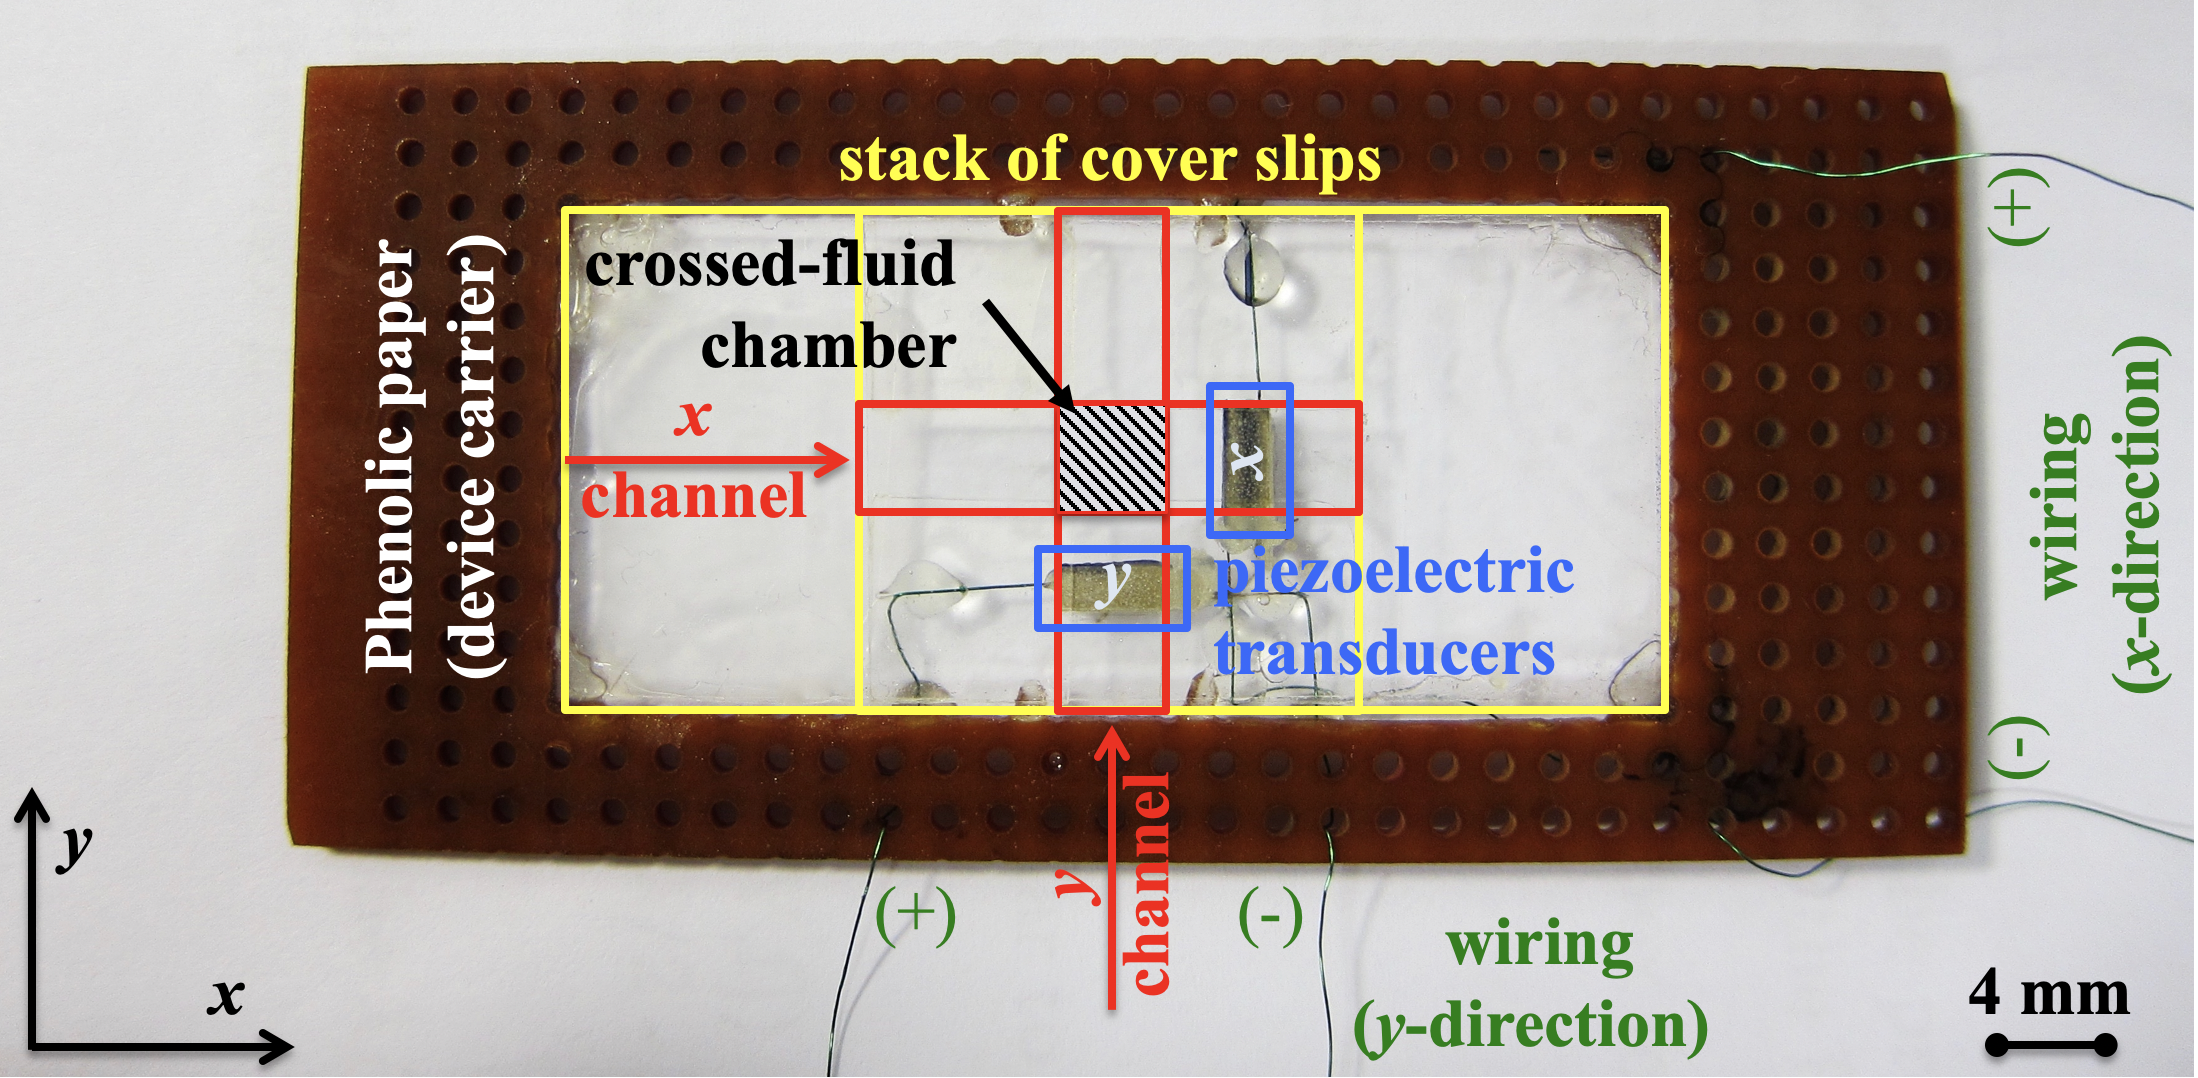
\includegraphics[width=84mm]{\relPath/10_Figures/Fig3.png}
    \caption{Stack of three coverslips form the device where the middle layer 
    includes two fluid channels (\SI{4.0x22}{\mm} with a depth of 
    \numrange{0.13}{0.17} \si{\milli\meter}, red boxes) in an orthogonal 
    arrangement. The two channels intersect and form a \SI{4.0x4.0}{\mm} crossed 
    chamber (black hatched area). Each piezo-electric transducer 
    \SI{4.0x2.0x0.5}{\mm} (PZ26, blue boxes) individually excites a direction.  
    The relative phase difference $\zeta$ of the excitation signals is freely 
    adjustable. The phenolic paper holds the stack and has the size of a 
    standard specimen slide for mounting.\label{fig:VT-Fig3}}
\end{figure}
%%%%%%%%%%%%%%%%%%%

Two piezo-electric transducers (Ferroperm, Pz26, $l$, $w$, and $h$ = \numlist{4; 
2; 1} \si{\mm}, Kvistgaard, Denmark) were glued on the stack of coverslips with 
conductive glue (EPOXY Technology, H20E, Billerica, MA, USA) perpendicular to 
each channel in $x$- and $y$-direction. The distance between the center of the 
fluidic chamber and each transducer was \SI{7}{\mm}. This distance was set such, 
that the microscope objective stays clear from the transducers. The resulting 
thin design of the device ensured the usage of the optical trap and decoupled 
the standing wave modes in the channels ($x$ and $y$). This specific design 
enabled controlled excitation of standing wave modes in the directions of $x$ 
and $y$ as well as an individual control of the excitation phase $\zeta$ (see 
\cref{fig:VT-Fig4}).

For our measurements we always used the same spatial position within the device.  
Hence, the rotation of the particles is always in the same direction for our 
experiments. However, \citeauthor{Lamprecht2015} \cite{Lamprecht2015} 
demonstrated how the rotation direction is dependent on the spatial location and 
the phase $\zeta$ of the two standing waves. In addition, in the supplemental 
material two videos are provided that show the change of rotation direction when 
changing these two parameters.

%%%%%%%%%%%%%%%%%%%
\begin{figure}
    \centering
    \includegraphics[width=84mm]{\relPath/10_Figures/Fig4.png}
    \caption{The device is filled with a water/glycerol (70$\%$/30$\%$) mixture 
    containing \SI{4}{\micro\meter} copolymer particles (Duke Scientific 
    Cooperation, Palo Alto, CA, USA) and it has two identical modes in $x$- and 
    $y$-direction at \SI{1.043}{\mega\hertz}. a) and b) depict the isolated 
    modes at \SI{15}{\Vrms} for the $x$- and $y$-direction, respectively. The 
    resulting measured wavelength $\lambda_{P}$ was approximately 
    \SI{1.4}{\milli\meter} for both directions.\ c) and d) show the particle 
    pattern for the two orthogonal standing waves inside the crossed-fluid 
    chamber at $\zeta= 0$ and $\zeta= \frac{\pi}{2}$, respectively. These 
    observations confirm the assumption of a 2 dimensional orthogonal standing 
    wave field.\label{fig:VT-Fig4}}
\end{figure}
%%%%%%%%%%%%%%%%%%%


\subsection{Particles \label{sec:VT-particles}}
For the visualization experiment in \cref{fig:VT-Fig4} we used \SI{4}{\micro\meter} 
copolymer particles (Duke Scientific Cooperation, Palo Alto, CA, USA). For the 
optical trapping experiments with single particles we used silica particles 
because they are more precise in their dimensions compared to polystyrene 
particles. In addition, they have better interactions
with the acoustical field. Moreover, the results of \citeauthor{Hahn2016} 
\cite{Hahn2016} suggest that in the region of $R \approx \delta$ and ratios of 
$\sfrac{\rho_{\text{s}}}{\rho_{\text{f}}}$ between 2 and 15 result a greater 
magnitude of the acoustic viscous torque results. With the used fluid ($\rho_{f} 
= \SI{1.1}{\gram\per\cubic\centi\meter}$) and our silica particles ($\rho_{s} = 
\SI{2.0}{\gram\per\cubic\centi\meter}$) the ratio 
$\sfrac{\rho_{\text{s}}}{\rho_{\text{f}}} \approx 1.8$.

In order to validate the proposed power spectrum method two sets of validation 
experiments are explained in \cref{sec:VT-rotationDetectionValidation}. For those 
the \SI{4.39}{\micro\meter} particles were modified differently for each 
experiment. We use this size of particles since they are better visible when 
simultaneously measuring the rotation with a camera. There was the need to 
\emph{mark} the spherical \SI{4.39}{\micro\meter} silica particles because a 
reliable rotation measurement with the camera of unmarked spherical particles 
was not possible.

Two methods for marking were used. In both cases the rotation could be easily 
tracked by optical microscopy because the particle size of 
\SI{4.39}{\micro\meter} silica glass micro-spheres (Microparticles
GmbH, Berlin, Germany) is much larger than the optical resolution.
For the set of experiments, silica particles were deformed between two polished 
metal plates by applying a pressure of \SI{1}{\mega\pascal} to achieve a slight 
degree of non-sphericalness (see \cref{fig:VT-Fig5}). For the second set, uncoated 
particles were distributed on a glass specimen slide (MENZEL GmbH, 
Menzel-Glaesser, Braunschweig, Germany) and coated by a Sputter coater (B7340 
Manual Sputter Coater, Van Loenen Instruments, Zaandam, Netherlands) with a gold 
coating (see \cref{fig:VT-Fig6}). After coating, the particles were half-covered 
with a \SIrange{10}{20}{\nano\meter} thick gold layer at their surface 
orientated to the gold electrode. The coating affected the acoustic properties 
not substantially. The particles showed, i.e., same trapping and rotational 
behavior within the acoustical trap. Averted particle surfaces showed a thinner 
gold layer of about \SIrange{0}{10}{\nano\meter}.

    \section{Experimental Procedure\label{sec:VT-experimentalProcedure}}

The observed time-averaged spatial off-set of the particles inside the optical 
trap is naturally zero, but the frequency content of the observed particle 
motion includes the thermal energy content of the particle as well as its 
rotational frequency. The angular frequency appears as an additional peak in the 
power spectrum of the rotating particle. In order to validate this detection 
method, particles with a rotational rate of less than \SI{1.66}{\hertz} 
(\SI{100}{\rpm}) were observed by a high-speed camera (HiSpec1 G2 Mono, Fastec, 
San Diego, USA) while also recording their power spectrum.  In the validation 
experiments the transparent device was filled with \SI{4.39}{\micro\meter} 
silica glass micro-spheres suspended in distilled water at a low concentration 
of a few particles per \si{\micro\liter}.  This low particle concentration does 
not effect the ratio $\tilde{\rho} = \sfrac{\rho_{\text{s}}}{\rho_{\text{f}}}$. 
The open channel ends were sealed with silicone oil to ensure a constant fluid 
volume during the measurements.

\subsection{Rotation Detection 
Validation\label{sec:VT-rotationDetectionValidation}}

Two sets of validation experiments were performed: (i) non-spherical particle 
rotation with slightly non-spherical particles; (ii) spherical particle rotation 
with gold covered particles for increased contrast in the video observation 
\cite{Lamprecht2013}. 

According to \citeauthor{Hahn2016} \cite{Hahn2016}, non-spherical objects can 
also be rotated due to the acoustic VT, but here effects of acoustic radiation 
torques may govern or influence their rotations \cite{Wang2012}. A slightly 
non-spherical \SI{4.39}{\micro\meter} silica particle (see \cref{fig:VT-Fig5}) was 
trapped in the optical potential well with \SI{100}{\milli\watt} laser power and 
moved to the reference position ($x,y,z = 0$) in the center of all three 
dimensions of the fluid chamber. The acoustic pressure field is formed by two 
orthogonal standing waves at the same excitation frequency of 
\SI{1090}{\kilo\hertz} and \SI{10.0}{\Vrms} amplitude. The particle was then 
optically moved to the closest resulting pressure node (intersection of two 
pressure nodal lines in $x$- and $y$-direction) with respect to the reference 
position. Positions of the pressure nodes were determined by a previous set of 
experiments.

The phase difference between the acoustic excitation directions $x$- and 
$y$-direction was set to $\zeta=\sfrac{\pi}{2}$, and the non-spherical particle 
rotated counter-clockwise with $\Omega = \SI{1.12}{\hertz}\,(\SI{67}{\rpm})$ 
(arithmetic mean of \SI{0.3}{\hertz} (\SI{18}{\rpm}) and \SI{1.6}{\hertz} 
(\SI{96}{\rpm}); see also \cref{fig:VT-Fig5}). At $\zeta=0$ the particle did not 
rotate because of the stable, non-varying acoustic potential.

%%%%%%%%%%%%%%%%%%%
\begin{figure}
    \centering
    \includegraphics[width=100mm]{\relPath/10_Figures/Fig5.png}
    \caption{Power spectral density and results of the video analysis of a 
      counter-clockwise rotating non-spherical silica particle at 
      \SI{1090}{\kilo\hertz} and \SI{10.0}{\Vrms} with relative phase shift of 
      $\zeta= \sfrac{\pi}{2}$. The 10 times averaged power spectrum of the 
      $y$-signal of the detection unit (QPD) was recorded with a frequency 
      resolution of $\Delta f = \SI{0.1}{\hertz}$ and a sampling rate of 
      \SI{1}{\MS}. Three main peaks were observed at \numlist{0.3; 0.8; 1.6} 
      \si{\hertz}. The frequency peak at \SI{0.8}{\hertz} corresponds to a 
      relative $xy$-motion of the trapped particle, whereas the peaks at 
      \numlist{0.3; 1.6} \si{\hertz} (\numlist{18;96} \si{\rpm}) are related to 
      a non-constant angular rotation $\Omega(\varphi)$ of the particle. The 
      measured results are in correlation with the determined rotational rate by 
      the high-speed video analysis with a frame rate of \SI{100}{\fps}. See the 
      supplemental material for a optically trapped particle rotating 
      sequentially with two velocities due to its imperfect spherical 
  shape.\label{fig:VT-Fig5}}
\end{figure}%
%%%%%%%%%%%%%%%%%%%

In \cref{fig:VT-Fig5}, the average of 10 power spectral density plots is depicted, 
each obtained from a \SI{10}{\second} recording. The frequency resolution is 
$\Delta f=\SI{0.1}{\hertz}$. Three main peaks were observed in the power 
spectrum at \numlist{0.3; 0.8; 1.6} \si{\hertz}, which correlate with the 
frequencies detected by the contemporaneous video detection. We see these peaks 
on both QPDs for the $x-$ and $y$-direction. However for some of the latter 
rotational measurements, the $xy$-motion of the particle adds more peaks 
depending on the major axis of the acoustic displacement. All other peaks are 
related to multiple repetitions of these angular frequencies due to deviations 
of the spherical shape of the particle.  The peak at \SI{0.8}{\hertz} 
corresponds to a relative $xy$-motion of the particle, whereas the peaks at 
\numlist{0.3; 1.6} \si{\hertz} are related to angular frequencies of the 
non-constant rotation $\Omega(\varphi)$ of the particle. The existence of two 
frequency peaks is related to the influence of different acoustic pressures in 
$x$ and $y$-direction because the amplitude were not yet matched for this 
validation.  Hence, the acoustic radiation forces on the particle have different 
magnitudes in $x$ and $y$-direction. So, the distribution of acoustic radiation 
pressure on the particle changes during its rotation and leads to an additional 
orientation dependent acoustic radiation torque.  The influence of acoustic 
radiation forces on particle orientations is a well-known effect for small 
non-spherical particles with $r \ll \lambda$ \cite{Konig1891,Garbin2015}, but 
this experiment shows that this influence is also large enough to influence the 
rotation by the acoustic VT.  Particles with a larger degree of 
non-sphericalness did not even start to rotate in this set of experiments. This 
is in agreement with the predictions of \citeauthor{Hahn2016} \cite{Hahn2016}, 
that the acoustic VT decreases with a higher degree of elliptical shape of the 
particles. In contrast, the acoustic radiation torque increases and hinders a 
constant rotation of the particle, if the symmetry of the experimental acoustic 
potential at $\zeta= \sfrac{\pi}{2}$ is imperfect.

Previously, optical traps formed by a linearly polarized laser have been applied 
to rotate anisotropic particles \cite{GutirezMedina2010}. However, this torque 
is dependent on the orientation of the anisotropic particle with respect to the 
polarization plane of the laser. If the laser power is high enough, the 
acoustically induced rotation can be inhibited because the anisotropic particle 
is optically locked to the polarization plane. For perfectly spherical particles 
without any shape anisotropy this optical torque vanishes 
\cite{Manzo2006,Friese1998}. We did not observe influences of optical forces on 
the final rotational velocities of the spherical particles because the 
determined velocities in the experiments were independent of the applied laser 
power. For our validation experiments with deformed and gold coated particles we 
did not investigate further the influence of the linearly polarized laser on the 
particles. This indicates that the applied acoustic torque was greater in 
magnitude than the optical torque.

Also, the experiments that are presented afterward show that the particle 
rotation is dominated by the acoustic field. By moving the particle through the 
flow cell or by changing the phase of the excitation signal, the rotation can be 
stopped, started and reversed (see \cref{fig:VT-Fig8} and the video in the 
supplemental material).

A closer investigation was not possible in our current experimental set-up 
because particles sank due to gravity if the laser was turned off. Observed 
rotations near fluid boundaries (bottom plate) are governed by influences of 
near-boundary effects, e.g.\ higher viscous drag, different acoustic scattering 
and streaming which would complicate an investigation of low laser powers on the 
particle rotation.

The second set of validation experiments employed spherical particles with a 
thin gold layer to increase the contrast for the video observation 
\cite{Lamprecht2013}. The additional gold layer changed the optical properties of 
the particles and led to a different optical trapping behavior in the 
experiments. Most of the particles could not be trapped optically because the 
gold layer reflected the incident laser light (\SI{785}{\nano\meter}) and the 
resulting optical scattering forces pushed the particles away from the laser 
focus \cite{Zhou2020,Ashkin1992,Svoboda1994}. The particle needs to be 
transparent for the wavelength of the laser, in order to enable trapping. 
However, due to statistical variations of the coating process some particles 
were optically trappable, since just a small portion of the surface was coated.  
And hence, just a small portion of the incoming laser was reflected. One example 
of an optically trapped particle with a constant and stable rotation is shown in 
\cref{fig:VT-Fig6}. The brighter regions at the surface of the particle arise from 
the reflected laser light due to the partial gold coating.  These regions 
rotated with the optically trapped particle due to the acoustic VT.\@ The 
angular change of reflected light on the particle surface was then determined by 
the QPDs of the optical detection unit and increased the signal strength by a 
factor of 100 with respect to uncoated particles. The recorded power spectrum of 
the $x$- and $y$-signals included the information about the angular frequency of 
the rotating particle.

An example for a recorded power spectrum of a rotating gold-layered 
\SI{4.39}{\micro\meter} silica particle at an acoustic excitation frequency of 
\SI{1090}{\kilo\hertz} and amplitude of \SI{2.5}{\Vrms} with a relative phase 
shift of $\zeta= \sfrac{\pi}{2}$ is depicted in \cref{fig:VT-Fig6}. A clear peak 
can be seen at \SI{1.3}{\hertz}. The determined rotational rate of the particle 
by video observations was \SI{1.31}{\hertz} (\SI{78.6}{\rpm}), which correlates 
with the measured peak at \SI{1.3}{\hertz} (\SI{78.0}{\rpm}).  A further 
variation of the acoustic excitation parameters (amplitude and relative phase) 
shifted the peaks in frequency as predicted by 
\cref{eq:VT-Eq1,eq:VT-AcGovEqConti} (results are not shown) 
\cite{Lamprecht2013}.

%%%%%%%%%%%%%%%%%%%
\begin{figure}
    \centering
    \includegraphics[width=100mm]{\relPath/10_Figures/Fig6.png}
    \caption{Power spectral density and results of the video analysis of a 
      counter-clockwise rotating gold-coated spherical \SI{4.39}{\micro\meter} 
      silica particle at \SI{1090}{\kilo\hertz} and \SI{2.5}{\Vrms} with 
      relative phase shift $\zeta= \sfrac{\pi}{2}$. The 10 times averaged power 
      spectrum of the $y$-signal of the detection unit (QPD) was recorded with a 
      frequency resolution of $\Delta f=\SI{0.1}{\hertz}$ and a sampling rate of 
      \SI{1}{\MS}. A clear peak at \SI{1.3}{\hertz} and two additional peaks at 
      \numlist{2.6; 3.9} \si{\hertz} were observed. The amplitudes of the 
      additional peaks were one order of magnitude smaller as the amplitude of 
      the peak at \SI{1.3}{\hertz}. The peak at \SI{1.3}{\hertz} correlates with 
  the determined rotational rate by the high-speed video analysis at a frame 
  rate of \SI{100}{\fps}.\label{fig:VT-Fig6}}
\end{figure}%
%%%%%%%%%%%%%%%%%%%

\subsection{Rotation of particles where $\normBdLayer \approx 
1$\label{sec:VT-rotationParticles}}

The determinations of the rotational rate with the power spectrum-method opened 
the possibility to measure fast rotations ($>\SI{25}{\hertz}$ (\SI{1500}{\rpm})) 
of particles with a radius $R$ about \SI{1}{\micro\meter}.  For such small 
particles the ratio of the thickness of the viscous boundary layer $\delta$ and 
the particle radius $R$ approaches 1 ($\normBdLayer \approx 1$) in the 
\si{\mega\hertz}-range (\SIrange{1}{10}{\mega\hertz}). The analytical formulas 
become invalid for the case that $\normBdLayer > \sfrac{1}{15}$ \cite{Hahn2016}.  
Particle rotations within the limit $\normBdLayer \approx 1$ were experimentally 
validated by an investigation of silica spheres with a \SI{2.06}{\micro\meter} 
(Microparticles GmbH, Berlin, Germany) diameter resuspended with a 
water/glycerol (70$\%$/30$\%$) mixture.  The viscosity $\mu_f$ of the aqueous 
glycerol solution was \SI{0.06}{\pascal\second} \cite{Jerome1968} with a 
determined density of \SI{1.1}{\gram\per\centi\meter\cubed} (dense knife, DMA 
35N, Anton Paar GmbH, Graz, Austria) and increased the thickness of the viscous 
boundary layer to approximately \SI{1.33}{\micro\meter} at an excitation 
frequency of \SI{1043}{\kilo\hertz} ($\lambda \approx \SI{1.4}{\mm}$). The 
normalized viscous boundary layer is therefore $\normBdLayer \approx 1.30$.

The optical trapping set-up was originally designed to measure the acoustic 
force and pressure amplitudes inside micro-fluidic channels and cavities 
\cite{Lakaemper2015,Lamprecht2016}. The same procedure was used here to measure 
the local acoustic pressure amplitudes inside the fluid chamber of the 
transparent micro-device. An accurate prediction of the acoustic pressure 
amplitudes $A_{X}$ and $A_{Y}$ of the two orthogonal standing waves was 
important to determine the strength of the acoustic VT by observing the 
steady-state rotational rate $\finalOmega$ of rotating particles.

Therefore, the local acoustic pressure amplitudes $A_{X}$ and $A_{Y}$ were 
individually measured in $x$- and $y$-direction by exciting only one transducer 
of the corresponding $x$- or $y$-direction, respectively. We measured the 
acoustic forces in all three dimensions ($x$, $y$, $z$) acting on the 
\SI{2.06}{\micro\meter}-particle inside the optical trapping potential. The 
spatial measurement range was $\pm \SI{0.55}{mm}$ in the $x$- and $y$-direction.  
The point $(\SI{0.21}{\mm}, \SI{0.22}{\mm})$, measured relatively to the middle 
of the fluid chamber, corresponded to the spatial position where a pressure 
nodal line in $x$- and $y$-direction overlapped.

The maximal force amplitudes at \SI{1043}{\kilo\hertz} were 
\SIrange{-96}{+25}{\femto\newton} for the $x$-direction and 
\SIrange{-32}{28}{\femto\newton} for the $y$-direction. The peak-to-peak value 
of the determined forces in $y$-direction was about two times weaker than in 
$x$-direction. This factor of 2 was used to calibrate the piezoelectric 
excitation amplitude to reach equal acoustic pressure amplitudes in both 
excitation directions.

The excitation amplitude $U_{el}$ is proportional with the acoustic pressure 
amplitude $A_{x,y}$ ($U_{el} \propto A_{x,y}$), whereas the acoustic radiation 
force $F_{ac}$ has a quadratic dependency of the acoustic pressure amplitudes 
$A_{x,y}$ ($F_{ac} \propto A_{x,y}^2$) \cite{Barnkob2010}. Therefore, the 
excitation amplitude of the piezoelectric transducer in $y$-direction was 
increased by a factor of $\sqrt{2}$ for all further investigations. The acoustic 
pressure amplitude $p_{a}$ was calculated via
%%%%%%%%%%%%%%%%%%%
\begin{equation}
\label{eq:VT-PressurePredictions}
p_{a}^{2} = \frac{F}{\pi\,R^{3}\,\kappa_{0}\,\Phi(f_{1},f_{2})} 
\frac{1}{k\,\sin(2k\,x)} =
\frac{F}{\pi\,R^{3}\,\kappa_{0}\,\Phi(f_{1},f_{2})} 
\frac{\lambda_{\text{p}}}{2\pi\,\sin(x\,\sfrac{4\pi}{\lambda_{\text{p}}})}
\end{equation}
%%%%%%%%%%%%%%%%%%%
where a 1-dimensional standing plane wave is assumed \cite{Settnes2012a}. $F$ is 
the force measured with the optical trap, $\lambda_{\text{p}}$ the wavelength of 
the pressure field, $k = \sfrac{2\pi}{\lambda_{\text{p}}}$ the wavenumber, $R$ 
the radius of the spherical particle, $\kappa_{0}$ the compressibility of the 
fluid, $\Phi(f_{1},f_{2})$ the so-called acoustic contrast factor, and 
$\sin(kx)$ the spatial dependency of the standing wave.  Since the force was 
measured at the force maximum $\sin(2\,kx)$ is set to $\sin(\sfrac{\pi}{2}) = 
1$. In addition, because of the value for the normalized viscous boundary layer 
$\normBdLayer \approx 1$, the corrected dipole factor  
$f_{2}(\tilde{\rho},\normBdLayer)$ of \citeauthor{Settnes2012} 
\cite{Settnes2012} was utilized. With this, the determined acoustic pressure 
amplitude for the standing wave in $x$-direction was \SI{245}{\kilo\pascal} for 
the measured acoustic forces and wavelength if an influence of acoustic 
streaming was neglected. 

After the calibration of the excitation amplitudes and the acoustic pressures of 
both acoustofluidic channels the acoustic VT was quantitatively investigated 
inside the fluid chamber. One \SI{2.06}{\micro\meter} silica particle was 
optically trapped and moved in $x$-direction inside the wave field of two 
orthogonal standing waves, while measuring its power spectrum at specified 
measurements points. The location of one specific pressure nodal line for an one 
dimensional standing wave in $x$- and $y$-direction at \SI{1043}{\kilo\hertz} 
was determined at $x=\SI{0.21}{\mm}$ and $y=\SI{0.22}{\mm}$, respectively. These 
nodal lines formed a local pressure node at their intersection if the acoustic 
excitation was shifted in phase with $\zeta = \sfrac{\pi}{2}$. There, the 
acoustic VT had its maximum value. Therefore, a measurement line in 
$x$-direction was defined between $x=0.20\pm0.55~\si{\milli\meter}$ at constant 
$y=\SI{0.22}{\milli\meter}$.

The particle exerted a counter-clockwise rotation at the local pressure node due 
to the acoustic VT at \SI{1043}{\kilo\hertz} with \SI{10.0}{\Vrms} and 
\SI{14.2}{\Vrms} excitation amplitude in $x$- and $y$-direction, respectively.

The detection of the angular frequency in a recorded power spectrum was not 
trivial for those small and spherical silica particles due to their low 
signal-to-noise ratios. Additionally, the power spectrum was disturbed by added 
frequencies of the acoustic excitation set-up; namely, an additional peak at 
\SI{100}{\hertz} originating from the voltage supply and \SI{170}{\hertz} from 
the amplifier itself.  Therefore, all measurements were repeated with a 
ten-times lower excitation amplitudes in $x$- and $y$-direction to calibrate the 
power spectrum measurements due to unknown influences of the environment and 
attached set-ups. An initialization of particle rotations was not observed at 
these low excitation amplitudes. A peak detection algorithm (implemented in 
MatLab) used the calibration measurement to eliminate disturbances on the 
determined power spectrum of a locally rotating particle due to VT.\@

\Cref{fig:VT-Fig8} depicts the power spectrum of a rotating particle with a clear 
peak at a frequency of \SI{165}{\hertz}. The particle was located at the 
relative location (-0.075, 0.220) \si{\mm} and its rotation was initialized at 
\SI{1043}{\kilo\hertz} with an excitation amplitude of \SI{10.0}{\Vrms} and 
\SI{14.2}{\Vrms} in $x$- and $y$-direction, respectively.  An appearance of 
additional peaks at a multiple of the angular frequency was not monitored by the 
peak-detection algorithm, likely because the amplitude of these peaks was below 
the noise floor. Their signal strength was expected to be one order of 
magnitude smaller (see \cref{fig:VT-Fig5,fig:VT-Fig6}).  The detection 
algorithm had a threshold value of 3 (signal-to-noise ratio) for indicating 
peaks in determined power spectrum.  \cref{fig:VT-Fig8}b depicts the 
corresponding calibration power spectrum of \cref{fig:VT-Fig8}a.

\Cref{fig:VT-Fig10} depicts the peaks detected by the peak-detection algorithm. 
Each point represents a separate rotational rate measurement. Interestingly, the 
strength of the angular frequency peaks was proportional to Brownian noise with 
$\sfrac{1}{f^2}$. These peaks are due to the particle rotations at positions 
within the spatial range of $x=0.21\pm\SI{0.55}{\mm}$ and $y=\SI{0.22}{\mm}$.  
The spatial dependency and formation of these peaks were in correlation with 
\cref{eq:VT-Eq1} and the maximal frequency $f$ of a peak in the power spectrum was 
\SI{229}{\hertz} ($ \finalOmega = \SI{13.8e3}{\rpm} $). The quantitative 
analysis revealed that maximal rotation appeared at $x=\SI{0.16}{\mm}$ (pressure 
node) and the resulting acoustic wavelength in $x$-direction was \SI{1.9}{\mm}.  
A one-dimensional wave in water at $f=\SI{1043}{\kilo\hertz}$ predicts an 
acoustic wavelength of $\lambda = \sfrac{c}{f} \approx \SI{1.4}{\mm}$ (compare 
\cref{fig:VT-Fig4}). The difference in wavelength from \cref{fig:VT-Fig4} 
($\lambda \approx \SI{1.4}{\mm} $) to the fitted value of $\lambda \approx 
\SI{1.9}{\mm} $ may be related to an off-set in orientation of the 
3-dimensional wavenumber $|\bm{k}|^{2} = k^{2}_{x} + k^{2}_{y} + k^{2}_{z}$ in 
the optical trapping set-up. Eigenfrequencies and their acoustic fields are 
influenced by the optical trapping set-up due to the additional interface 
between the acoustofluidic device and the water-immersion objective 
\cite{Lamprecht2016}.  \Cref{fig:VT-Fig4} was observed with a standard 
microscope lens that did not need to have an immersion oil layer on top of the 
device.

%%%%%%%%%%%%%%%%%%%
\begin{figure}
    \centering
    \includegraphics[width=100mm]{\relPath/10_Figures/Fig9.png}
    \caption{a) Measured power spectrum of an optically trapped 
    \SI{2.06}{\micro\meter} particle that rotated counter-clockwise due to the 
    acoustic VT at \SI{1043}{\kilo\hertz} with \SI{10.0}{\Vrms} and 
    \SI{14.2}{\Vrms} excitation amplitude in $x$- and $y$-direction, 
    respectively. The particle was located at (-0.075, 0.220) \si{\mm}. The 
    spectrum of the $x$-signal (QPD) was recorded and 10 times averaged with a 
    frequency resolution of $\Delta f=\SI{1}{\hertz}$ and a sampling rate of 
    \SI{1}{\MS}. A clear signal peak due to particle rotation at 
  \SI{165}{\hertz} was observed with a signal-to-noise ratio of about 5. The 
signal peak at \SI{110}{\hertz} is related to influences of the acoustic 
excitation set-up.\ b) Control measurement of a non-rotating optically trapped 
\SI{2.06}{\micro\meter} particle under acoustic excitation at 
\SI{1043}{\kilo\hertz} with \SI{1}{\Vrms} and \SI{1.42}{\Vrms} excitation 
amplitude in $x$- and $y$-direction, respectively. A particle rotation was not 
initialized at these low excitation amplitudes and these recorded power spectrum 
of non-rotating \si{\micro\meter} particles were used to identify the peaks not 
related to particle rotation power spectrum due to influences of the environment 
and the acoustic excitation set-up. The peak at \SI{110}{\hertz} is related to 
amplifier noise and vanished when the acoustic excitation set-up was turned off 
\cite{Lamprecht2016}.\label{fig:VT-Fig8}}
\end{figure}
%%%%%%%%%%%%%%%%%%%

%%%%%%%%%%%%%%%%%%%
\tikzsetnextfilename{VT_results}
\begin{figure}[tb]
  \centering
  \includegraphics[]{Plots/cache/VT_results.eps}
    % \begin{tikzpicture}
    %     \begin{axis}
    %         [scale only axis,
    %         width = 89mm,
    %         height = 5cm,
    %         xtick = {-0.5,-0.25,0,0.25,0.5},
    %         xmin = -0.55, xmax = 0.55,
    %         ymax = 280, ymin = -5,
    %         xlabel = {Realative x position [\si{\mm}]},
    %         ylabel = {power spectrum Peak Frequency [\si{\hertz}]}]

    %         \addplot[red,thick,mark size=4pt,only marks,mark=x] table[x=y, 
    %         y=f,col sep=comma] {\relPath/40_Fitting/datapoints.dat};

    %         \addplot[thick,blue,dashed] table[x=y, y=f,col sep=comma] 
    %         {\relPath/40_Fitting/datapointsFit.dat};

    %         \node[blue,above] at (axis cs: 0.16,229) 
    %         {$\left|229.18\,\sin\left(3.30\,X_{i} + 1.03 \right)\right|$};

    %     \end{axis}
    % \end{tikzpicture}
    \caption{Spatial dependency of frequency peaks (red) due to the acoustic VT 
      from the power spectrum-method. Multiple power spectra of a 
      \SI{2.06}{\micro\meter} silica particle were recorded at specific 
      measurement points in $x$-direction at $x=\SI{0.21}{\mm}\pm\SI{0.5}{\mm}$ 
      and $y=\SI{0.22}{\mm}$. The acoustic field formed two orthogonal standing 
      waves in $x$- and $y$-direction at \SI{1043}{\kilo\hertz} with a relative 
      phase shift of $\zeta =\frac{\pi}{2}$. The determined frequency peaks were 
      fitted to the equation $\left|c_{1}\,\sin(c_2\,X_i + c_3)\right|$ (dashed 
      blue).  The resulting maximal frequency $f$  from the fit was 
      \SI{229}{\hertz} ($ \finalOmega = \SI{13.8e3}{\rpm}$) and the determined 
      acoustic wave in $x$-direction $\lambda_{X}=\sfrac{2\pi}{c_2}$ was 
    \SI{1.90}{\mm}. The pressure nodal point with maximal rotational rate was 
  determined at $x=\SI{0.16}{\mm}$, whereas zero VT was determined at 
$x=\SI{-0.31}{\mm}$ (pressure anti-node).\label{fig:VT-Fig10}}
\end{figure}
%%%%%%%%%%%%%%%%%%%

    \section{Conclusion\label{sec:VT-conclusion}}

The combination of an optical trap and a transparent VT device opened the 
possibility to measure the VT independently of the acoustic radiation force. The 
power spectrum analysis provided the quantitative information about the angular 
frequency $\Omega$. Unwanted effects related to close proximities of walls near 
the rotating particle and influences of oscillating micro gas bubbles were 
avoided.  The optically levitated particle ensured a largely unaffected rotation 
due to the acoustic VT.\@ 

Moving the stage of the optical set-up changed the rotation direction of a 
trapped and rotated particle between two neighboring pressure nodes because of 
the acoustic VT \cite{Lamprecht2015} (see the supplemental material for a 
particle rotation in different directions depending on the spatial location 
inside the wave field).  These kinds of experiments were so far unattainable in 
a continuous manner and for unstable acoustic particle positions (positive 
acoustic contrast factor) of zero VT.\@

The validation experiments showed that the detected additional peaks in the 
measured power spectrum are directly related to the rotational rate of the 
particle rotation. The detected signals had peaks at multiples of this peak 
frequency.  However, for transparent silica particles with an almost perfectly 
spherical shape the amplitudes of the multiples were too small to overcome the 
signal-to-noise-ratio. The high-speed video analysis is limited by the camera's 
frame rate. In contrast, the detection bandwidth of the optical trap easily 
spans tens of \si{\kilo\hertz}. As already mentioned, optical trapping has some 
unique advantages to investigate the acoustic VT: 1) Allows to probe almost  any 
spatial position within the acoustofluidic device. 2) Measures rotational 
frequencies up to multiple \si{\kilo\hertz}. 3) Works with conventional, non 
coated, spherical particles. 4) Frequencies are directly visible in the data (no 
need for post processing of video data).

In order to calculate the theoretical rotational rate $\finalOmega$ of the 
particle, the local acoustic pressure amplitude needs to be known in advance.  
Because of that, a local acoustic pressure amplitude analysis was carried out 
before the rotation detection experiments. Depending on the calculation 
approach, different results are obtained for the rotational rate. The analytical 
calculation for the final rotational rate $\finalOmega$ (see \cref{eq:VT-Eq1}) 
\cite{Lamprecht2015, Busse1981, Rudnick1977, Wang1989} with a dynamic fluid viscosity of 
$\mu_{f} = \SI{0.06}{\pascal\second}$ led to rates between 
\SIrange{613}{811}{\hertz} (\SIrange{36.8e3}{48.7e3}{\rpm}). The numerical 
calculations of \citeauthor{Hahn2016} \cite{Hahn2016} yield a final rotational 
rate for a \SI{2.06}{\micro\meter} silica particle with $\normBdLayer=1.30$ of 
\SIrange{208}{277}{\hertz} (\SIrange{12.5e3}{16.6e3}{\rpm}) at room temperature 
(\SI{25}{\celsius}).  The first value for the rotational rate corresponds each 
time to the theoretical wavelength of $\lambda \approx \SI{1.4}{\mm}$ (see 
\cref{fig:VT-Fig4}) and acoustic pressure amplitude $p_{a}\left(\lambda\right) = 
\SI{245}{\kilo\pascal} $; the latter to the measured $\lambda \approx 
\SI{1.9}{\mm}$ (see \cref{fig:VT-Fig10}) and $p_{a}\left(\lambda\right) = 
\SI{282}{\kilo\pascal} $. The disagreement between our experiments and 
\cref{eq:VT-Eq1} is regarding the equilibrium state for the final rotational rate 
$\finalOmega$. The spatial dependency of \cref{eq:VT-Eq1} ($\cos\left(k\,X\right), 
\cos\left( k\,Y \right)$) agrees with our experiments.

In contrast to that, the power spectrum-method estimates the steady-state 
rotational rate $\finalOmega$ to \SI{229}{\hertz} (\SI{13.8e3}{\rpm}). This 
value is very close to the numerically obtained values (about 10$\%$ higher for 
$\lambda \approx \SI{1.4}{\mm}$ or 17$\%$ lower for $\lambda \approx 
\SI{1.9}{\mm}$).  These deviations can be in part explained by a decrease of 
the fluid viscosity due to laser-induced heating (up to \SI{2}{\kelvin}) in 
close proximity of the laser focus \cite{Peterman2003}. Since the measured force 
of our trap scales with $\sqrt{\mu}$ and the viscosity variation around 
\SI{25}{\celsius} is relatively small, the temperature induced measurement 
errors are about 2\%.  This slightly changes the acoustic pressure amplitudes 
with respect to the calibrated pressure of \SI{245}{\kilo\pascal} ($\lambda 
\approx \SI{1.4}{\mm}$) or \SI{282}{\kilo\pascal} ($\lambda \approx 
\SI{1.9}{\mm}$) because the investigated pressure node was located slightly off 
the calibration lines.  Also, the in oil immersed lens of the optical trap 
changes the theoretical (pure) 1-dimensional acoustic field to a 3-dimensional.

The experiment clearly showed that the analytical calculations of 
\citeauthor{Lamprecht2015,Busse1981, Rudnick1977, Wang1989} \cite{Lamprecht2015, Busse1981, 
Rudnick1977, Wang1989}  overestimate the rotational velocities at ratios $\normBdLayer 
\approx 1$. Furthermore, the complexity and spatially varying torques on 
\si{\micro\meter} particles were measured, whereas the simulations are limited 
to the ideal case of plane-standing waves and incompressible particles in an 
infinitely large fluid domain. 

A further application of the acoustic torque analysis with an optical trap could 
be the experimental determination of the influence of the particle density on 
the acoustic VT.\@ Particles with the same density can show different rotational 
directions at a fixed point in the acoustic field, if the ratio $\normBdLayer$ 
changes \cite{Hahn2016}.

Optical torques on double refracting quartz particles is a possible tool to 
directly measure acoustic torques \cite{La2004}. The laser power of such 
modulated optical traps could be used to calibrate acoustic torques on trapped 
particles at equilibriums where the optical torque counteracts the acoustic 
torque. 

% \vspace*{7mm}

% A.L and C.G. contributed equally to this work.



% BibTeX users please use one of
% \bibliographystyle{iopart-num}
\bibliographystyle{unsrtnat}
% \printbibliography
\bibliography{alle_referenzen.bib} 

\end{document}
